%11_graphs.tex
%notes for the course PandA2 COMS10001 taught at the University of Bristol
%2016-7 Conor Houghton conor.houghton@bristol.ac.uk

%To the extent possible under law, the author has dedicated all copyright 
%and related and neighboring rights to these notes to the public domain 
%worldwide. These notes are distributed without any warranty. 

\documentclass[11pt,a4paper]{scrartcl}
\typearea{12}
\usepackage{graphicx}
\usepackage{listings}
\usepackage{tikz}
\usepackage{tikz-qtree}
\usetikzlibrary{positioning}
%\usetikzlibrary{arrows.meta}
\lstset{language=C}
\pagestyle{headings}
\markright{COMS10001 - PandA2 11\_graphs - Conor}
\begin{document}

\subsection*{11- graphs\footnote{\texttt{http://github.com/conorhoughton/COMS10001}}}

\begin{figure}
\begin{center}
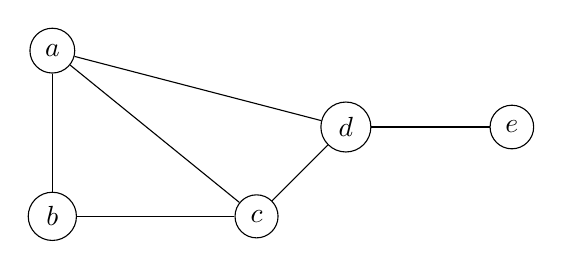
\begin{tikzpicture}
\node[draw,circle](a){$a$};
\node[draw,circle, below = 1.5cm of a](b){$b$};
\node[draw,circle, right =2cm of b](c){$c$};
\node[draw,circle, above right = 1cm of c](d){$d$};
\node[draw,circle, right = 1.5cm of d](e){$e$};
\path (a) edge (b);
\path (b) edge (c);
\path (c) edge (d);
\path (d) edge (e);
\path (a) edge (d);
\path (c) edge (a);
\end{tikzpicture}
\end{center}
\caption{A graph. \label{fig:graph}}
\end{figure}

\begin{equation}
[A_{ij}]=\left(
\begin{array}{ccccc}
0&1&1&1&0\\
1&0&1&0&0\\
1&1&0&1&0\\
1&0&1&0&1\\
0&0&0&1&0
\end{array}
\right)
\end{equation}


\begin{figure}
\begin{center}
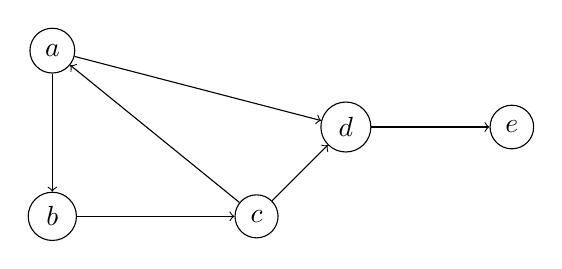
\begin{tikzpicture}
\node[draw,circle](a){$a$};
\node[draw,circle, below = 1.5cm of a](b){$b$};
\node[draw,circle, right =2cm of b](c){$c$};
\node[draw,circle, above right = 1cm of c](d){$d$};
\node[draw,circle, right = 1.5cm of d](e){$e$};
\path (a) edge[->] (b);
\path (b) edge[->] (c);
\path (c) edge[->] (d);
\path (d) edge[->] (e);
\path (a) edge[->] (d);
\path (c) edge[->] (a);
\end{tikzpicture}
\end{center}
\caption{A directed graph. \label{fig:dir_graph}}
\end{figure}

\begin{figure}
\begin{center}
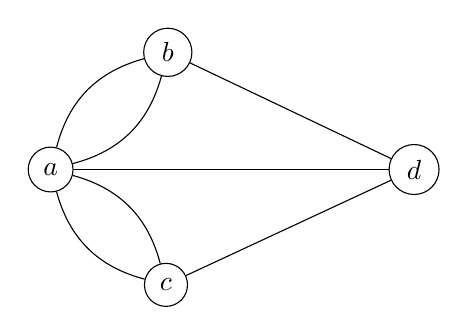
\begin{tikzpicture}
\node[draw,circle](a){$a$};
\node[draw,circle, above right = 1.5cm of a](b){$b$};
\node[draw,circle, below right = 1.5 cm of a](c){$c$};
\node[draw,circle, right = 4cm of a](d){$d$};
\path (a) edge[-,bend right] (b);
\path (a) edge[-,bend left] (b);
\path (a) edge[-,bend right] (c);
\path (a) edge[-,bend left] (c);
\path (a) edge[-] (d);
\path (d) edge[-] (b);
\path (d) edge[-] (c);
\end{tikzpicture}
\end{center}
\caption{The Bridges of K\"{o}nigsberg graph. \label{fig:konigsberg_graph}}
\end{figure}





\end{document}
